%%%% Time-stamp: <2012-08-20 17:41:39 vk>

%% example text content
%% scrartcl and scrreprt starts with section, subsection, subsubsection, ...
%% scrbook starts with part (optional), chapter, section, ...
\chapter{Implementation}
\label{sec:impl}
The theory in the previous chapters was partially acquired during the research phase but mostly during the implementation of the packages. 
The basics in these chapters are not adjusted to the particular use in this project, furthermore they cover parts which are implicitly used. 
Therefore this section focuses on the implementational details of the single packages and subpackages fitting the described theory to the 
implementational approach.

\section{Communication}
\label{sec:comm}
One of the main functionalities needed by both tools is the communication between the device and the USB port it is attached to. Although this does not relate 
to OBD in particular, it is a common requirement in software projects which are either distributed (distributed systems) or such which are 
meant for standardized distributions (Linux, Windows, Mac) in combination with external hardware. This implementation uses the ELM$327$ v$1.4$/v$1.5$ \cite{ELM} 
as external hardware. The goal of the communication middleware package (see \nameref{sec:tecspec}) is to provide development tools for simple access 
to the ELM chip without consideration to specifics of the port (USB, COM etc.). Another requirement which falls into this category is the emulation 
of a given USB ELM device to enable testing of OBD tools, leading to the implementation of a virtual USB FTDI device and controlling its behaviour.

The implementation of this package is based on the knowledge acquired in the chapter \nameref{sec:USB} and \nameref{sec:CSaB}.

\subsection{Serial Communication}
\label{sec:serialComm}
After acquiring an overview of the general OBD functionality and familiarizing with the ELM$327$ the next step was trying the terminal program 
Screen \cite{SCREEN} on GNU/Linux. It enables the user to send hexadecimal coded commands to any mounted device, in this case the ELM, and receives its responses, 
more concretely the diagnostic trouble code data. The screen starting command looks as follows:

\begin{verbatim}
sudo screen /dev/ttyUSB0 <baud rate> 
\end{verbatim}

The ELMs communication baud rate is $38400$ bits per seconds. Sending the ELM command ATZ causes the device to respond with its description, shown in \myfigref{fig:screen_response}.
%\nameref{fig:screen_response} ~\ref{fig:screen_response}

\myfig{screen}%% filename w/o extension in the folder figures
 {width=\textwidth}%% maximum width/height, aspect ratio will be kept
 {Screen showing the Response of ELM ATZ Command}%% caption
 {Figure}%% optional (short) caption for list of figures
 {fig:screen_response}%% label

As visible on the image above Screen still has issues with carriage returns.

Naturally the next step is to try requesting trouble codes which is simply accomplishable using Screen. An ignition coil failure can be
caused by simply removing the ignition coil's power supply of the testvehicle. The response of the requested temporary DTC equals the anticipated 
ignition coil failure code as hexadecimal value. 

%TODO: PICTURE
% \myfig{screen}%% filename w/o extension in the folder figures
%  {width=\textwidth}%% maximum width/height, aspect ratio will be kept
%  {Screen showing the Response of ELM ATZ Command}%% caption
%  {Screen Terminal Screenshot}%% optional (short) caption for list of figures
%  {fig:screen_response}%% label

The different open source libraries, like libusb \cite{LIBUSB}, bring the capability of getting all devices and their information like vendor and product ID.
Furthermore a simple algorithm searching the sysfs of Linux provides the associated terminal file path (/dev/tty…). Last but not least the 
operations of reading and writing are achieved by the simple file descriptor system calls read and write in combination with termios for 
setting the baud rate of these operations. 

USB normally does not offer the ability of defining baud rates. This issue originated from the need of FTDI devices for RS-$232$ ports. Therefore most
external hardware, like Arduino, based on such microcontrollers integrate a RS-$232$ to USB converter requesting a communication baud rate. Additional 
research revealed the libftdi library, used exactly for these serial communication issues with USB. It combines functionalities of libusb with serial
configurations like setting the baud rate. 

The usage of libftdi was momentarily discarded, due to no apparent benefit and the additional disadvantage of refactoring the already existing 
code. The needed functionality was already covered by combining the libusb package with TTY Linux driver and file descriptors as well as giving more
flexibility for function development in future releases.

\subsection{Emulation}
\label{sec:emulation}
The first approach consists of exploiting the USBIP API, which provides the functionality of sharing USB devices over a network. After 
assessing its feasibility the option of using its base library libusb-vhci proves to be more effective.

The VHCI project can be described as a driver. VHCI \cite{VHCI} (Virtual Host Controller Interface) is a kernel module with the capability of emulating an 
USB hardware device to the kernel. Kernel modules are code modules executed in the kernel space. They need to be compiled on each Linux kernel 
independently to match its structure. Furthermore the functionalities defined by kernel modules have to be executed with root privileges.

Although compiling the kernel module on each Linux distribution individually and executing the emulation as root can be rated as a disadvantage,
it is capable of freely emulating USB devices and using the full scope of USB features defined in the \citetitle{USB} \cite{USB}. 

The already existing example code of the project emulates a simple HID (Human Interface Device) which mostly covers the needs of the project. 
Nevertheless, gradually refactoring the example code leads to an emulation of an FTDI device. The result is comprised of three classes 
representing the emulation, visualized in \myfigref{fig:classdiagram_communication}:

\begin{itemize}
 \item USBEmulationSupervisor
 \item USBRequestHandler
 \item EmulatedDevice
\end{itemize}

The supervisor handles the general setup of the VHCI structure, including work requests and distribution of different USB functionalities as 
well as the request handler. The request handler’s responsibility lies with parsing the USB requests and storing them in an instance of 
“EmulatedDevice” and responding accordingly to the request. Currently only one emulated device is possible at a time. The emulated device holds 
the device-, configuration- and language descriptors as well as the function pointer defining the callback. This callback is meant for giving 
free possibility of defining what shall happen on a specific command. Especially ELM commands are of interest since OBD commands are 
standardised. The implementation covers only the most essential functionalities of the VHCI library.

The inconvenience of needing administrator rights discourages the utilization of the emulation. This issue is unavoidable, since libusb and 
libusb\_vhci both use functionalities, like claiming a hardware device, which require administrator rights. The fully functional software is 
intended to have its superuser\-id\-bit (suid) set once, therefore granting it administrator rights by default or at least ensuring that it has to be executed 
as administrator.

\myfig{classdiagram_communication}%% filename w/o extension in the folder figures
 {width=\textwidth}%% maximum width/height, aspect ratio will be kept
 {Classdiagram oft the Communication Emulation}%% caption
 {Figure}%% optional (short) caption for list of figures
 {fig:classdiagram_communication}%% label

\section{Databases}
\label{sec:database}
Storing and managing data is bound to become an issue due to the enormous amount of data sets in relation to OBD. Therefore a thoroughly 
implemented database interface cannot be avoided. For reasons of simplicity MySQL is chosen as base query language for the database. The main 
advantages leading to the choice of MySQL are the easy installation of MySQL server and client on all Linux distributions as well as the API 
availability. MySQLConnector++ \cite{MYSQL} is a C++ API for MySQL, which supplies the basic framework for executing and parsing responses of any database. 
Since it is an external library \nameref{sec:CleanCode} advises to wrap its API in a self defined interface, which is represented by this subpackage. 

The general structure composes of a class responsible for dispatching the requests, a class for parsing the data into a C++ conform class 
structure as well as an executor class defining the insertion and deletion commands, as shown in \myfigref{fig:classdiagram_database}. Keeping the philosophy 
of test driven development (see \nameref{sec:XP}) in mind it seems wise to setup a test database as an SQL dump and supply a script reinitiating the database. 
After the manipulation of the database by a unit test this script can be used to reset the test database to its initial state. 
\myfig{classdiagram_database}%% filename w/o extension in the folder 
 {width=\textwidth}%% maximum width/height, aspect ratio will be kept
 {Classdiagram showing the Database Package}%% caption
 {Figure}%% optional (short) caption for list of figures
 {fig:classdiagram_database}%% label

The configuration parameters can either be entered hardcoded or by parsing an XML file containing the host address, user, password and database 
name. The parsing structure is thoroughly explained in the \nameref{sec:configuration}. The XML looks as follows:

\begin{verbatim}
 <?xml version="1.0" encoding="UTF-8"?>
 <!DOCTYPE database SYSTEM "database.dtd">
 <database>
   <address>127.0.0.1</address>
   <user>obd</user>
   <password></password>
   <dbname>OBD_TroubleCodes</dbname>
 </database>
\end{verbatim}

The password field is left empty as the user obd has no password set up.

\section{OBD Base}
\label{sec:obdbase}
The OBDBase package represents the OBD specific part of this thesis. It provides links between the OBD structures like hexadecimal responses 
from the ELM to the database entries with their column definitions and IDs, as well as calculations, minimum and maximum values of single 
sensors and ELM specific command representations.

The OBD interface responds to PIDs of service mode I and II with a certain amount of bytes. This amount is defined in the ISO $15031$ \cite{ISO15031} depending 
on the sensor the PID represents. Every $32$nd PID is a request to get the implementation status of the next $32$ PIDs. Meaning 
PID $0$, which equals the OBD command $01$ $00$, returns four bytes where each bit is interpreted as a boolean value, stating the availability of the corresponding PID. The 
interpretation of these received bytes is defined in the ISO standard as well. Analyzing the accessible PIDs a clustering into four different value types can be extracted.

\subsection{Calculation Values}
Calculation values are responses or part of a response, where the received value represents the quantity of the PID’s underlying entity. 
As the name suggests there are additional calculations necessary. The standard defines the environment parameters of these value which are 
supplied by an XML file. PID $0x66$ is an example of a calculation value:

\begin{verbatim}
 <value interpretation="calculation">
  <name>MAF Sensor A</name>
  <bytes>2</bytes>
  <min>0</min>
  <max>2047.96875</max>
  <unit>g/s</unit>
 </value>
\end{verbatim}

These definitions describe the range of the received data, in this case from $0-2047.96875$ g/s for $0-65535$ decimal value of two bytes. 
This means that a received byte value $0$ corresponds to $0$ g/s and a decimal value of $65535$ represents $2047.9687$ g/s. When resolving these 
relations the following formula can be used for converting values: 

\[ c_s = \frac{max - min}{2^{no. bits} - 1} \]

\[ v_{interpreted} = v_{raw} * c_s + min \]

Those formulas are reflected in the following listing:

\begin{verbatim}
 void OBDCalculationValue::
   interpretCalculationValue(std::vector<uint8_t> input)
 {
   unsigned int compound_value = calculateCompoundValue(input);
   double scale = (max_-min_)/(pow(2.0, byte_amount_*8.0)-1);
   interpreted_value_ = compound_value * scale + min_;
   uninterpreted_value_ = compound_value;
 }
\end{verbatim}

The conversion of interpreted values to raw values naturally deduces:

\[ v_{raw} = \frac{(v_{interpreted} - min)}{c_s} \]

\begin{verbatim}
 void OBDCalculationValue::
   interpretCalculationByteArray(double value)
 {
   interpreted_value_ = value;
   interpreted_value_ = std::min(interpreted_value_, max_);
   interpreted_value_ = std::max(interpreted_value_, min_);
   double scale = (max_-min_)/(pow(2.0, byte_amount_*8.0) - 1);
   uninterpreted_value_ = (interpreted_value_ - min_) / scale;
 }
\end{verbatim}

\subsection{Value Mapping Values}

This type describes raw values which are used on a predefined mapping to get a string representation of this corresponding PID's request. Meaning the 
value directly maps to a result string. The configuration of such a value requires only the mapping itself, as illustrated by the PID $0x5F$:

\begin{verbatim}
 <value interpretation="mapping">
  <bytes>1</bytes>
  <mapping type="value">
   <entry from="0E">LKW (Euro IV) B1</entry>
   <entry from="0F">LKW (Euro V) B2</entry>
   <entry from="10">LKW (Euro EEV) C</entry>
  </mapping>        
</value>
\end{verbatim}

\subsection{Bit Mapping Values}

As the name suggests the bit mapping type describes values where each bit has a different meaning. In this case the only information required from the ISO is 
the mapping. In some cases a bit's true and false value signify different outputs for the same entity. An example of such a value is PID $0$ as well as PID $0x65$:

\vbox{
\begin{verbatim}
 <value interpretation="mapping">
  <bytes>1</bytes>
  <mapping type="bit">
   <entry from="0" set="false">Kraftaufnahme inaktiv</entry>
   <entry from="0" set="true">Kraftaufnahme aktiv</entry>
   <entry from="1" set="false">
     Automatikgetriebe in Park-/Neutralstellung</entry>
   <entry from="1" set="true">
     Vorwärts- oder Rückwärtsgang</entry>
   <entry from="2" set="false">
     Manuelles Getriebe in … Kupplung getreten</entry>
   <entry from="2" set="true">Gang eingelegt</entry>
   <entry from="3" set="false">Vorglühlampe aus</entry>
   <entry from="3" set="true">Lampe ein</entry>
  </mapping>
 </value>
\end{verbatim}}

The ``from'' field specifies the bit position while the ``set'' is an optional attribute to assign a bit's value to a concrete output. In this 
case it is supplied, meaning that depending on the bits status different strings are mapped. If the ``set'' attribute is not explicitly stated it 
is assumed true.

\begin{verbatim}
 std::string OBDBitMappingValue::
   interpretToValue(std::vector<uint8_t> input)
 {
   interpreted_value_ = calculateCompoundValue(input);
   uninterpreted_value_ = interpreted_value_;
   return getInterpretedValueAsString();
 }
\end{verbatim}

As this code shows, in case of mapping values, the interpreted and uninterpreted values are identical and represent the key of the underlying mapping.

\subsection{Bit Combination Value Mapping}

This value parsing is a bit comparator mapping of more than two bits. The ``from'' field specifies the bit positions and the ``set'' represents the 
value it needs to equal to get the result string in question. PID $0x70$ is an example of such a mapping.

\begin{verbatim}
 <value interpretation="mapping">
  <bytes>1</bytes>
  <mapping type="bitcombination">
   <validitybit from="01">2</validitybit>
   <entry from="01" set="01">
     Offener Kreislauf, kein Fehler</entry>
   <entry from="01" set="10">
     Geschlossener Kreislauf, kein Fehler</entry>
   <entry from="01" set="11">
     Fehler vorhanden, Wert unzuverlässig</entry>
   <validitybit from="23">5</validitybit>
   <entry from="23" set="01">
     Offener Kreislauf, kein Fehler</entry>
   <entry from="23" set="10">
     Geschlossener Kreislauf, kein Fehler</entry>
   <entry from="23" set="11">
     Fehler vorhanden, Wert unzuverlässig</entry>
    </mapping>    
 </value>
\end{verbatim}

The first three entries correspond to the zeroth and first bit in combination. If they equal $1(0b01) \vee 2(0b10) \vee 3(0b11)$ the mapped string is selected.
The same principle is applied for the entries regarding the second and third bit combination.

\subsection{Inner Workings}

Since most PIDs do not consist of only one value or type, values have to be defined in the order they are supposed to be received. They can be 
combined as needed, so that multiple calculation values can be followed by any mapping value or vice versa. The total byte amount, resulting from the
addition of each value's byte length, is expected when parsing the OBD command's answer. This promotes significance to the order of the sequence in which the 
values are defined in the XML file.

Furthermore special OBD commands exist where the first byte defines which of the transmitted following bytes are valid values. These OBD 
commands are mostly used for array sensor PIDs. The package offers the optional definition of an automatic or manual validity mapping.

A validity mapping contains one or more bytes at the beginning of the response. The positioning of the bits correspond to the following bytes and 
their value. Each bit indicates the validity of the associated value.

There are no rules without exceptions. Certain values have a complex validity mapping structure especially in association with the bit 
combination mapping. The need for a manually configurable validity mapping emerges which leads to a differentiation of validity mapping 
modes (manual and auto). The amount of such values is limited to one or two occurrences. The manual mode requires definition of the validity bit position
for each tag. The following listing supplies an example:

\vbox{
\begin{verbatim}
 <obdcommand>
  <pid>70</pid>
  <description>Ladedruckregelung</description>
  <validitymapping  mode="manual">true</validitymapping>
  <values>
   <value interpretation="calculation">
    <name>Soll Ladedruck A</name>
    ...
    <validitybit>0</validitybit>    
   </value>
   <value interpretation="calculation">
    <name>Soll Ladedruck B</name>
    ...
    <validitybit>1</validitybit>    
   </value>
   ...
   <value interpretation="mapping">
    <bytes>1</bytes>
    <mapping type="bitcombination">
     <validitybit from="01">2</validitybit>
     <entry from="01" set="01">
       Offener Kreislauf, kein Fehler</entry>
     <entry from="01" set="10">
       Geschlossener Kreislauf, kein Fehler</entry>
     <entry from="01" set="11">
       Fehler vorhanden, Wert unzuverlässig</entry>
     <validitybit from="23">5</validitybit>
     <entry from="23" set="01">
       Offener Kreislauf, kein Fehler</entry>
    </mapping>        
   </value>
  </values>
 </obdcommand>
\end{verbatim}}
\pagebreak

High abstraction is achieved with the abstract base class OBDCommandValues. It defines main utility functions like adding bytes to a compound value, storing the 
raw and interpreted data and delegating the interpretation trough a pure virtual function to its derived classes. 

A simple factory pattern \cite{PATTERN}, which creates OBDCommandValues from its XML representation, ensures simple usability. It manufactures the values depending on 
the ``interpretation'' attribute of each ``value'' tag's definition and returns an abstract object representing the value. 

\subsection{ELM Commands}
\label{sec:ELM}
There is a set of ELM specific commands configurable for the communication to the control unit of the automobile. Generally the emulation has to 
answer those requests and the OBD tool must configure the ELM specific settings. Therefore it seems necessary to implement a parsing and object 
representation of the ElmCommands \cite{ELMDATASHEET} for our middleware package, see \nameref{sec:tecspec}.

The difficulty of this part of the OBDBase package surfaced when inspecting the single commands more closely. The ELM datasheet offers 
an inconsistent way of defining additional values. In most cases they are referenced as ``h'' (hexadecimal value) but there are some values 
referenced by ``x'', ``y'' or ``z'' as well.

\begin{verbatim}
 <command>
  <version>1.0</version>
  <elmcommand>"AL"</elmcommand>
  <description>"Allow Long (>7 byte) messages"</description> 
  <group>"OBD"</group>
 </command>
\end{verbatim}

\section{Configuration}
\label{sec:configuration}
The configuration subpackage is used to parse and write XML files. Currently there are following configuration files: 

\begin{itemize}
 \item elmcommandconfiguration.xml
 \item obdcommand.xml
 \item obdcuConfiguration.xml
 \item obdtoolConfiguration.xml
 \item dbconfiguration.xml
\end{itemize}

These contain configuration parameters for the software. The command configurations, elmcommandconfiguration.xml and odbcommand.xml, contain all 
commands known by the ELM$327$ extracted from its datasheet and all OBD commands consisting of service ID with its corresponding PID and name. 
The project configurations, obdcuConfiguration.xml and obdtoolConfiguration.xml, are only path declarations to the other configurations enabling 
factory resets.

This package uses the functionalities of the libxml++ \cite{XMLLIB} library. This library uses the Document Object Model (DOM) and supplies functionalities 
for parsing an XML file into a DOM model as well as writing a DOM model to a file. 

The base of the configuration package consists of the XMLWriter, XMLReader and DefaultHandler classes as visualized in \myfigref{fig:configuration_classdiagram}. 
Their purpose is to parse a DOM object into internal class representations, as suggested in \nameref{sec:CleanCode}, therefore simplifying the usage of the 
libxml++ library functions to creating a derived class of the DefaultXMLHandler. 

\myfig{classdiagram_configuration}%% filename w/o extension in the folder figures
 {width=\textwidth}%% maximum width/height, aspect ratio will be kept
 {Classdiagram of the Configuration Package}%% caption
 {Figure}%% optional (short) caption for list of figures
 {fig:configuration_classdiagram}%% label

This class has a pure virtual method handleNode which gets a xmlpp::Node* as parameter. A derived class instance can distinguish its execution 
and parsing behavior by comparing the name of the xmlpp::Node. The DefaultXMLHandler supplies protected functions for parsing 
xmlpp::TextNode* into C++ strings or setting xmlpp::TextNode* from C++ strings. 

Handlers only define the handling of the nodes, more precisely setting or parsing the underlying libxml++ DOM representation (xmlpp::Document). 
The XMLWriter and XMLReader classes are initialized with an instance of the DefaultXMLHandler. Its parse or write function requires an already 
existing XML file. Each function calls its internally defined DefaultHandler’s handleNode function while recursively iterating through DOM nodes. 
A well formed structure of the underlying XML files is ensured by the required DTD files defining the structure of the XML files, as shown in the following listing:

\begin{verbatim}
 <?xml version="1.0" encoding="UTF-8"?>
 <!DOCTYPE database SYSTEM "database.dtd">

 <database>
  <address>127.0.0.1</address>
  <user>obd</user>
  <password></password>
  <dbname>OBD_TroubleCodes</dbname>
 </database>
\end{verbatim}

\begin{verbatim}
 <!ELEMENT database (address, user, password, dbname)>
 <!ELEMENT address (#PCDATA)>
 <!ELEMENT user (#PCDATA)>
 <!ELEMENT password (#PCDATA)>
 <!ELEMENT dbname (#PCDATA)>
\end{verbatim}

The difference between the two classes is that, whilst the XMLReader only iterates and lets the handler save the read data, the XMLWriter sets 
the DefaultHandler into a mode, where he instead of parsing the node’s data sets it. After the iteration the XMLWriter writes to the same file 
it read from with the newly filled data.

% \begin{figure}[h!]
%  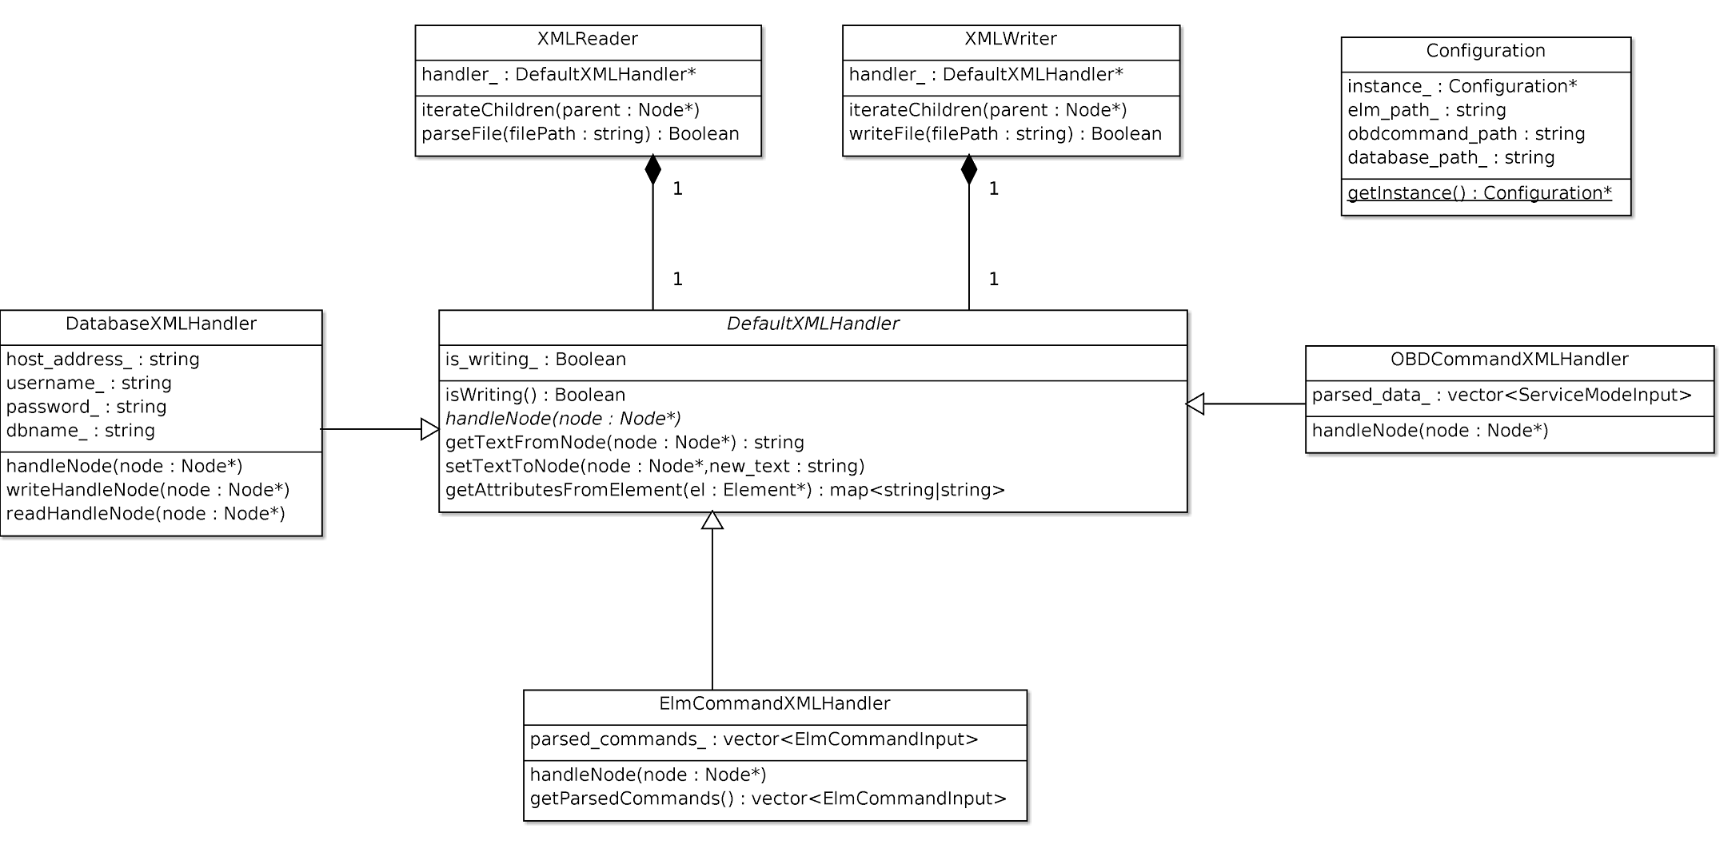
\includegraphics[width=\paperwidth]{figures/classdiagram_configuration}
%  \caption{Classdiagram of the configuration package}
% \end{figure}

%% vim:foldmethod=expr
%% vim:fde=getline(v\:lnum)=~'^%%%%\ .\\+'?'>1'\:'='
%%% Local Variables: 
%%% mode: latex
%%% mode: auto-fill
%%% mode: flyspell
%%% eval: (ispell-change-dictionary "en_US")
%%% TeX-master: "main"
%%% End: 